\documentclass[UTF8]{ctexart}
\usepackage{setspace}
\usepackage[letterpaper,top=2cm,bottom=2cm,left=3cm,right=3cm,marginparwidth=1.75cm]{geometry}
\CTEXsetup[format={\Large\bfseries}]{section}
\usepackage{amsmath}
\usepackage{mathabx}
\usepackage[mathscr]{eucal}
\usepackage{graphicx}

\title{Numerical Analysis HW3}

\author{数学与应用数学2002 王锦宸 }
\date{November 2022}

\begin{document}

\maketitle

\section*{Problem I}
\noindent From the definition of s(x). We know that p(x) should satisfy:
$$p(0) = 0\quad p(1) = 1\quad p'(1) = -3\quad p''(1) = 6$$
Use Hermite Interpolation, we have,
$$p(x) = 7x^3 - 18x^2 + 12x$$
To plus, it is not natural since $s''(x) = -36 \neq 0$

\section*{Problem II}
\subsection*{(a)}
Since we need a quadratic spline $s \in S_{2}^1$, we need two conditions.

\subsection*{(b)}
\noindent Denote $K_i = f[x_i,x-{i+1}]$, the table of divided difference is,
\begin{equation}
    \begin{array}{c|ccc}
        x_{i} & f_{i} & & \\
        x_{i} & f_{i} & m_{i} & \\
        x_{i+1} & f_{i+1} & K_{i} & \frac{K_{i}-m_{i}}{x_{i+1}-x_{i}}
    \nonumber
    \end{array}
\end{equation}

\noindent Then $p_i(x) = f_i + (x-x_i)m_i+(x-x_i)^2\frac{K_i-m_i}{x_{i+1}-x_i}$

\subsection*{(c)}
\noindent From (b), we know that $m_i = p_i'(x_i)$

\section*{Problem III}
\subsection*{(a)}
\noindent We have $$s(-1) = 1,s(0) = 1+c , s(1) = 1 + 8c$$ and $$s'(-1) = 0, s'(0) = 3c $$ and $$s''(1) = 0, s''(0) = 6c$$ from direct computation.\\
\noindent To be a natural cubic spline, we want $s''(1) = s''(-1) = 0.$\\
\noindent Assume that $s_2(x) = \alpha x^3+\beta x^2+\gamma x+\theta$ , then we need,
\begin{equation}
    \left\{\begin{array}{l}
        \theta=1+c \\
        \gamma=3 c \\
        2 \beta=6 c \\
        6 \alpha+2 \beta=0
    \nonumber
    \end{array}\right.
\end{equation}
\noindent Thus $s_2(x) = -cx^3 + 3cx^2+3cx+1+c$.

\subsection*{(b)}
\noindent If$s(1) = -1$, we have,
$$-c*1^3+3c*1^2+3c*1+1+c = -1$$
Thus $c=-\frac{1}{3}$.

\section*{Problem IV}
\subsection*{(a)}
\noindent $\text { Since } f=\cos \left(\frac{\pi}{2} x\right) \text {, then } f^{\prime}(x)=-\frac{\pi}{2} \sin \left(\frac{\pi}{2} x\right), f^{\prime \prime}(x)=-\left(\frac{\pi}{2}\right)^{2} \cos \left(\frac{\pi}{2} x\right) \text {. }$
Thus, we have,
\begin{equation}
    \left\{\begin{array}{l}
         f(-1) = 0,\;f(0)=1,\;f(1)=0 \\
         f'(-1) = -\frac{\pi}{2},\;f'(0)=0,\;f'(1) = -\frac{\pi}{2}\\
         f''(-1)=0,\;f''(0)=1,\;f''(1)=0
    \nonumber
    \end{array}\right.
\end{equation}
The interpolation of knots -1, 0 ,1 is,
\begin{equation}
    s(x)=
    \left\{\begin{array}{ll}
        -\frac{1}{2} x^{3}-\frac{3}{2} x^{2}+1 & \text { if } x \in[-1,0] \\
        \frac{1}{2} x^{3}-\frac{3}{2} x^{2}+1 & \text { if } x \in[0,1]
    \nonumber
    \end{array}\right.
\end{equation}

\subsection*{(b)}
\noindent From (a) we can get,\\
\begin{equation}
    s(x) = \left\{\begin{array}{l}
        -3x-3 \text{ if } x\in [-1,0]\\
        3x-3 \text{ if } x\in [0,1]
    \nonumber
    \end{array}\right.
\end{equation}
Thus, $\int_{-1}^{1}\left[s^{\prime \prime}(x)\right]^{2} d x=6$

\noindent (i) If g(x) be the quadratic polynomial, $\int_{-1}^{1}\left[g^{\prime \prime}(x)\right]^{2} d x = 8 > 6$.\\
(ii) If $g(x) = cos(\frac{\pi}{2}x), g''(x) = -\frac{\pi ^2}{4}cos(\frac{\pi}{2}x)$. Thus $\int_{-1}^{1}\left[g^{\prime \prime}(x)\right]^{2} d x = \frac{\pi^4}{16} > 6$.

\section*{Problem V}
\subsection*{(a)}
\noindent From the textbook, we know that the recursive definition is,
$$B_{i}^{n+1}(x)=\frac{x-t_{i-1}}{t_{i+n}-t_{i-1}} B_{i}^{n}(x)+\frac{t_{i+n+1}-x}{t_{i+n+1}-t_{i}} B_{i+1}^{n}(x)$$
and the initial condition is,
\begin{equation}
    B_{i}^{0}(x) = \left\{\begin{array}{ll}
        1 & \text { if } x \in\left(t_{i-1}, t_{i}\right] \\
        0 & \text { otherwise }
    \nonumber
    \end{array}\right.
\end{equation}
Thus, we have,
\begin{equation}
    B_{i}^{2}(x) = \left\{\begin{array}{lr}
        \frac{\left(x-t_{i-1}\right)^{2}}{\left(t_{i+1}-t_{i-1}\right)\left(t_{i}-t_{i-1}\right)} & \text { if } x \in\left(t_{i-1}, t_{i}\right] \\
        \frac{\left(x-t_{i-1}\right)\left(t_{i+1}-x\right)}{\left(t_{i+1}-t_{i-1}\right)\left(t_{i+1}-t_{i}\right)}+\frac{\left(t_{i+2}-x\right)\left(x-t_{i}\right)}{\left(t_{i+2}-t_{i}\right)\left(t_{i+1}-t_{i}\right)} & \text { if } x \in\left(t_{i}, t_{i+1}\right] \\
        \frac{\left(t_{i+2}-x\right)^{2}}{\left(t_{i+2}-t_{i}\right)\left(t_{i+2}-t_{i+1}\right)} & \text { if } x \in\left(t_{i+1}, t_{i+2}\right] \\
        0 & \text { otherwise }
    \nonumber
    \end{array}\right.
\end{equation}  

\subsection*{(b)}
We can get $\frac{d}{dx} B^2_i(x)$ from direct computation,
\begin{equation}
    \frac{d}{d x} B_{i}^{2}(x) = \left\{\begin{array}{lr}
    \frac{2\left(x-t_{i-1}\right)}{\left(t_{i+1}-t_{i-1}\right)\left(t_{i}-t_{i-1}\right)} & \text { if } x \in\left(t_{i-1}, t_{i}\right] \\
    \frac{t_{i-1}+t_{i+1}-2 x}{\left(t_{i+1}-t_{i-1}\right)\left(t_{i+1}-t_{i}\right)}+\frac{t_{i}+t_{i+2}-2 x}{\left(t_{i+2}-t_{i}\right)\left(t_{i+1}-t_{i}\right)} & \text { if } x \in\left(t_{i}, t_{i+1}\right] \\
    \frac{-2\left(t_{i+2}-x\right)}{\left(t_{i+2}-t_{i}\right)\left(t_{i+2}-t_{i+1}\right)} & \text { if } x \in\left(t_{i+1}, t_{i+2}\right] \\
    0 & \text { otherwise }
    \nonumber
    \end{array}\right.
\end{equation}

\noindent When $x = t_i$,
$$\lim_{x -> t_i^-} \frac{d}{dx}B_i^2(x) = \frac{2}{t_{i+1}-t_{i-1}},\quad \lim_{x -> t_i^+} \frac{d}{dx}B_i^2(x) = \frac{2}{t_{i+1}-t_{i-1}}$$
also, when $x = t_{i+1}$,
$$\lim_{x -> t_i^-} \frac{d}{dx}B_i^2(x) = \frac{-2}{t_{i+2}-t_{i}},\quad \lim_{x -> t_i^+} \frac{d}{dx}B_i^2(x) = \frac{-2}{t_{i+2}-t_{i}}$$
Thus, it continues at $x = t_i \text{ and } x = t_{i+1}$.
\subsection*{(c)}
\noindent When $x \in (t_{i-1}, t_i]$,  there is no $x^*$ satisfying $\frac{d}{dx}B_i^2(x^*) = 0$.
When $x \in (t_{i}, t_i{i+1}$, we have,
$$x^{*}=\frac{t_{i+2} t_{i+1}-t_{i} t_{i-1}}{t_{i+2}+t_{i+1}-t_{i}-t_{i-1}}$$
\noindent satisfying $\frac{d}{dx}B_i^2(x^*) = 0$.

\subsection*{(d)}
\noindent From the expression of $\frac{d}{dx}B_i^2(x)$ and (c), we know that $B_i^2(x)$ reach it extremes at $x = x^*, t_{i-1},t_{i+2}$.\\
$\text {Since } B_{i}^{2}\left(t_{i-1}\right)=B_{i}^{2}\left(t_{i+2}\right)=0, \text { and } B_{i}^{2}\left(x^{*}\right)=\frac{t_{i+2}-t_{i-1}}{t_{i+2}+t_{i+1}-t_{i}-t_{i-1}}<1 \text{, } B_{i}^{2} \in [0,1)$.

\subsection*{(e)}
Take $i = 0,\dots,4$ as an example,

\begin{figure}[htp]
    \centering
    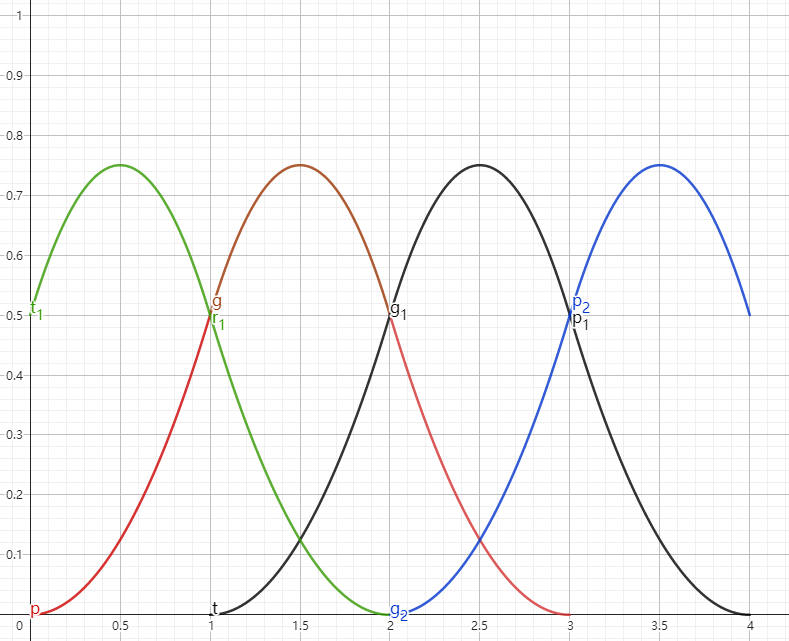
\includegraphics[width=10cm]{plot1.png}
    \caption{Plot of $B_i^2(x)$}
    \label{fig:1L}
\end{figure}



\section*{Problem VI}
\noindent Let's construct the table of divided difference to verify the Theorem.\\
1° when $x \in (t_{i-1}, t_{i}],$
\begin{equation}
    \begin{array}{c|ccc}
    t_{i-1} & 0 & & \\
    t_{i} & \left(t_{i}-x\right)^{2} & \frac{\left(t_{i}-x\right)^{2}}{t_{i}-t_{i-1}} & & \\
    t_{i+1} & \left(t_{i+1}-x\right)^{2} & t_{i+1}+t_{i}-2 x & \frac{t_{i+1}+t_{i}-2 x-\frac{\left(t_{i}-x\right)^{2}}{t_{i}-t_{i-1}}}{t_{i+1}-t_{i-1}} & \\
    t_{i+2} & \left(t_{i+2}-x\right)^{2} & t_{i+2}+t_{i+1}-2 x & 1 
    \nonumber
    \end{array}
\end{equation}

\noindent Thus,
\begin{equation}
    \begin{aligned}
        \left(t_{i+2}-t_{i-1}\right)\left[t_{i-1}, t_{i}, t_{i+1}, t_{i+2}\right](t-x)_{+}^{2} &= 1-\frac{t_{i}+t_{i+1}-2 x-\frac{\left(t_{i}-x\right)^{2}}{t_{i}-t_{i-1}}}{t_{i+1}-t_{i-1}}\\ 
        &= \frac{\left(x-t_{i-1}\right)\left(x-t_{i-1}\right)}{\left(t_{i+1}-t i-1\right)\left(t_{i}-t_{i-1}\right)}\\ 
        &= B_i^2(x)
    \nonumber    
    \end{aligned}
\end{equation}

\noindent 2° when $x \in (t_{i},t_{i+1}],$
\begin{equation}
    \begin{array}{c|ccc}
    t_{i-1} & 0 & \\
    t_{i} & 0 & 0 & \\
    t_{i+1} & \left(t_{i+1}-x\right)^{2} & \frac{\left(t_{i+1}-x\right)^{2}}{t_{i+1}-t_{i}} & \frac{\left(t_{i+1}-x\right)^{2}}{\left(t_{i+1}-t_{i}\right)\left(t_{i+1}-t_{i}\right)} \\
    t_{i+2} & \left(t_{i+2}-x\right)^{2} & \frac{\left(t_{i+2}-x\right)^{2}-\left(t_{i+1}-x\right)^{2}}{t_{i+2}-t i+1} & \frac{\frac{\left(t_{i+2}-x\right)^{2}-\left(t_{i+1}-x\right)^{2}}{t_{i+2}-t i+1}-\frac{\left(t_{i+1}-x\right)^{2}}{t_{i+1}-t_{i}}}{\left(t_{i+2}-t_{i}\right)}
    \nonumber
    \end{array}
\end{equation}
\noindent Thus,
\begin{equation}
   \begin{aligned}
        \left(t_{i+2}-t_{i-1}\right)\left[t_{i-1}, t_{i}, t_{i+1}, t_{i+2}\right](t-x)_{+}^{2}&=\frac{\frac{\left(t_{i+2}-x\right)^{2}-\left(t_{i+1}-x\right)^{2}}{t_{i+2}-t i+1}-\frac{\left(t_{i+1}-x\right)^{2}}{t_{i+1}-t_{i}}}{\left(t_{i+2}-t_{i}\right)}-\frac{\left(t_{i+1}-x\right)^{2}}{\left(t_{i+1}-t_{i}\right)\left(t_{i+1}-t_{i}\right)}\\ &=\frac{\left(x-t_{i-1}\right)\left(t_{i+1}-x\right)}{\left(t_{i+1}-t_{i-1}\right)\left(t_{i+1}-t_{i}\right)}+ \frac{\left(t_{i+2}-x\right)\left(x-t_{i}\right)}{\left(t_{i+2}-t_{i}\right)\left(t_{i+1}-t_{i}\right)}\\
        &= B_i^2(x)
    \nonumber
   \end{aligned}
\end{equation}

\noindent 3° when $x \in (t_{i+1},t_{i+2}],$
\begin{equation}
    \begin{array}{c|ccc}
    t_{i-1} & 0 & \\
    t_{i} & 0 & 0 & \\
    t_{i+1} & 0 & 0 & 0 \\
    t_{i+2} & \left(t_{i+2}-x\right)^{2} & \frac{\left(t_{i+2}-x\right)^{2}}{t_{i+2}-t i+1} & \frac{\left(t_{i+2}-x\right)^{2}}{\left(t_{i+2}-t_{i}\right)\left(t_{i+2}-t_{i+1}\right)}
    \nonumber
    \end{array}
\end{equation}
\noindent Thus,
\begin{equation}
    \begin{aligned}
        \left(t_{i+2}-t_{i-1}\right)\left[t_{i-1}, t_{i}, t_{i+1}, t_{i+2}\right](t-x)_{+}^{2} &= \frac{\left(t_{i+2}-x\right)^{2}}{\left(t_{i+2}-t_{i}\right)\left(t_{i+2}-t_{i+1}\right)}\\
        &= B_i^2(x)
    \nonumber    
    \end{aligned}
\end{equation}

\noindent 4° when $x \in (-\infty, t_{i-1}]$ or $x \in (t_{i+2}, \infty)$,\\
it is obvious that $\left(t_{i+2}-t_{i-1}\right)\left[t_{i-1}, t_{i}, t_{i+1}, t_{i+2}\right](t-x)_{+}^{2}=0$.

\section*{Problem VII}
\noindent According to the theory of derivative of B-Splines, we have,
$$\frac{d}{d x} B_{i}^{n}(x)=\frac{n B_{i}^{n-1}(x)}{t_{i+n-1}-t_{i-1}}-\frac{n B_{i+1}^{n-1}(x)}{t_{i+n}-t_{i}}$$
Hence,
\begin{equation}
    \begin{aligned}
        & \int_{t_{i-1}}^{t_{i+n-1}} \frac{B_{i}^{n}(x)}{t_{i+n-1}-t_{i-1}} d x-\int_{t_{i}}^{t_{i+n}} \frac{B_{i+1}^{n}(x)}{t_{i+n}-t_{i}} d x \\
        =& \int_{t_{i-1}}^{t_{i+n-1}}\left[\frac{B_{i}^{n}(x)}{t_{i+n}-t_{i-1}}-\frac{B_{i+1}^{n}(x)}{t_{i+n}-t_{i}}\right] d x \\
        =&\left.\frac{1}{n} B_{i}^{n+1}(x)\right|_{t_{i-1}} ^{t_{i+n}} \\
        =& 0
    \nonumber
    \end{aligned}
\end{equation}
\noindent Thus, It holds independent of the index i and it has nothing to do with whether the spacing of the knots is uniform

\section*{Problem VIII}
\subsection*{(a)}
\noindent Let establish the chart of divided difference,
\begin{equation}
    \begin{array}{l|ccc}
    x_{i} & x_{i}^{4} & \\
    x_{i+1} & x_{i+1}^{4} & x_{i+1}^{3}+x_{i+1}^{2} x_{i}+x_{i+1} x_{i}^{2}+x_{i}^{3} \\
    x i+2 & x_{i+2}^{4} & x_{i+2}^{3}+x_{i+2}^{2} x_{i+1}+x_{i+2} x_{i+1}^{2}+x_{i+1}^{3} & x_{i+2}^{2}+x_{i+1}^{2}+x_{i}^{2}+x_{i} x_{i+1}+x_{i+1} x_{i+2}+x_{i+2} x_{i}
    \nonumber
    \end{array}
\end{equation}
Thus, we have,
$$\tau_{2}\left(x_{i}, x_{i+1}, x_{i+2}\right)=x_{i} x_{i+1}+x_{i+1} x_{i+2}+x_{i+2} x_{i}+x_{i+2}^{2}+x_{i+1}^{2}+x_{i}^{2}=\left[x_{i}, x_{i+1}, x_{i+2}\right] x^{4}$$

\subsection*{(b)}
\noindent By the lemma of the recursive definition, we have,
$$\tau_{k+1}\left(x_{1}, \cdots, x_{n}, x_{n+1}\right)=\tau_{k+1}\left(x_{1}, \cdots, x_{n}\right)+x_{n+1} \tau_{k}\left(x_{1}, \cdots, x_{n}, x_{n+1}\right)$$
Thus, we can derive,
\begin{equation}
    \begin{aligned}
    &\left(x_{n+1}-x_{1}\right) \tau_{k}\left(x_{1}, \ldots, x_{n}, x_{n+1}\right) \\
    =& \tau_{k+1}\left(x_{1}, \ldots, x_{n}, x_{n+1}\right)-\tau_{k+1}\left(x_{1}, \ldots, x_{n}\right)-x_{1} \tau_{k}\left(x_{1}, \ldots, x_{n}, x_{n+1}\right) \\
    =& \tau_{k+1}\left(x_{2}, \ldots, x_{n}, x_{n+1}\right)-\tau_{k+1}\left(x_{1}, \ldots, x_{n}\right)
    \nonumber
    \end{aligned}
\end{equation}

\noindent By induction,\\
When n = 0, $\tau_{m}\left(x_{i}\right)=\left[x_{i}\right] x^{m}$
Now assume that the recursive formula is true for every n < m, consider n+1,
\begin{equation}
    \begin{aligned}
    & \tau_{m-n-1}\left(x_{i}, \cdots, x_{i+n+1}\right) \\
    =& \frac{\tau_{m-n}\left(x_{i+1}, \cdots, x_{i+n+1}\right)-\tau_{m-n}\left(x_{i}, \cdots, x_{n}\right)}{x_{i+n+1}-x_{i}} \\
    =& \frac{\left[x_{i+1}, \cdots, x_{i+n+1}\right] x^{m}-\left[x_{i}, \cdots, x_{i+n}\right] x^{m}}{x_{i+n+1}-x_{i}} \\
    =& {\left[x_{i}, \cdots, x_{i+n+1}\right] x^{m} }
    \nonumber
    \end{aligned}
\end{equation}
\noindent Hence, it's proved.
\end{document}

